\section{Recovery Limit under Quality Degradation}
\label{appendix:recovery_limit}

Experiment~03 (\S\ref{sec:eval_catastrophic}) demonstrates recovery from an ${\sim}18$\% quality degradation within the standard 608-prompt Phase~3 horizon.  Here we characterise the \emph{recovery envelope}: the maximum degradation severity from which the system can recover to near-Phase~1 performance, and how extending the recovery horizon shifts that boundary.

\paragraph{Setup.}
We sweep Mistral-Large's degraded reward from $0.05$ to $0.85$ (4--94\% degradation relative to its normal reward of ${\sim}0.92$) using the quality-degradation protocol from Experiment~03: cost remains unchanged during Phase~2 so only the reward signal reveals the regression.  All runs use the moderate budget ($\$6.62{\times}10^{-4}$/prompt), 20~seeds, and the same hyperparameters as the main experiment.  We define \emph{full recovery} as a Phase~3/Phase~1 reward ratio ${\geq}97$\%.

\paragraph{Recovery envelope (Figure~\ref{fig:recovery_limit}a).}
At the standard 608-prompt horizon, full recovery is achieved for degradations up to ${\sim}18$\% (failure reward ${\geq}0.75$).  Beyond this threshold, recovery plateaus around 90--92\% regardless of severity: once the mean-estimate corruption exceeds what geometric forgetting and staleness-driven exploration can erase within 608~prompts, additional severity has diminishing marginal impact.

Extending Phase~3 to 1,800~prompts (${\sim}3{\times}$ the standard horizon) uniformly lifts the entire envelope.  Degradations up to ${\sim}44$\% now cross the 97\% full-recovery threshold, and even at 66\% degradation the system reaches 96.5\%.  For the most severe degradations (77--94\%), the extended horizon still improves recovery from ${\sim}90$\% to ${\sim}95$\%, but a floor emerges: once corruption is deep enough, the additional 1,200~prompts yield diminishing returns, suggesting that yet longer horizons or explicit operator intervention would be needed.

\paragraph{Convergence dynamics (Figure~\ref{fig:recovery_limit}b).}
The extended-horizon time-series reveal that recovery is monotonic but rate-dependent on severity.  A 21\% degradation converges to the Phase~1 baseline within ${\sim}600$ prompts, while a 66\% degradation requires the full 1,800~prompts and still falls just short.  In all cases the confidence bands narrow over time, indicating stable convergence rather than high-variance oscillation.

\paragraph{Deployment implications.}
For typical silent regressions (${\leq}20$\%), ParetoBandit's default configuration recovers automatically within the standard observation window.  For severe regressions, operators can either extend the recovery horizon or intervene with an explicit model demotion---the staleness-inflation mechanism ensures the demoted arm will be re-explored once conditions improve.

\begin{figure}[t]
\centering
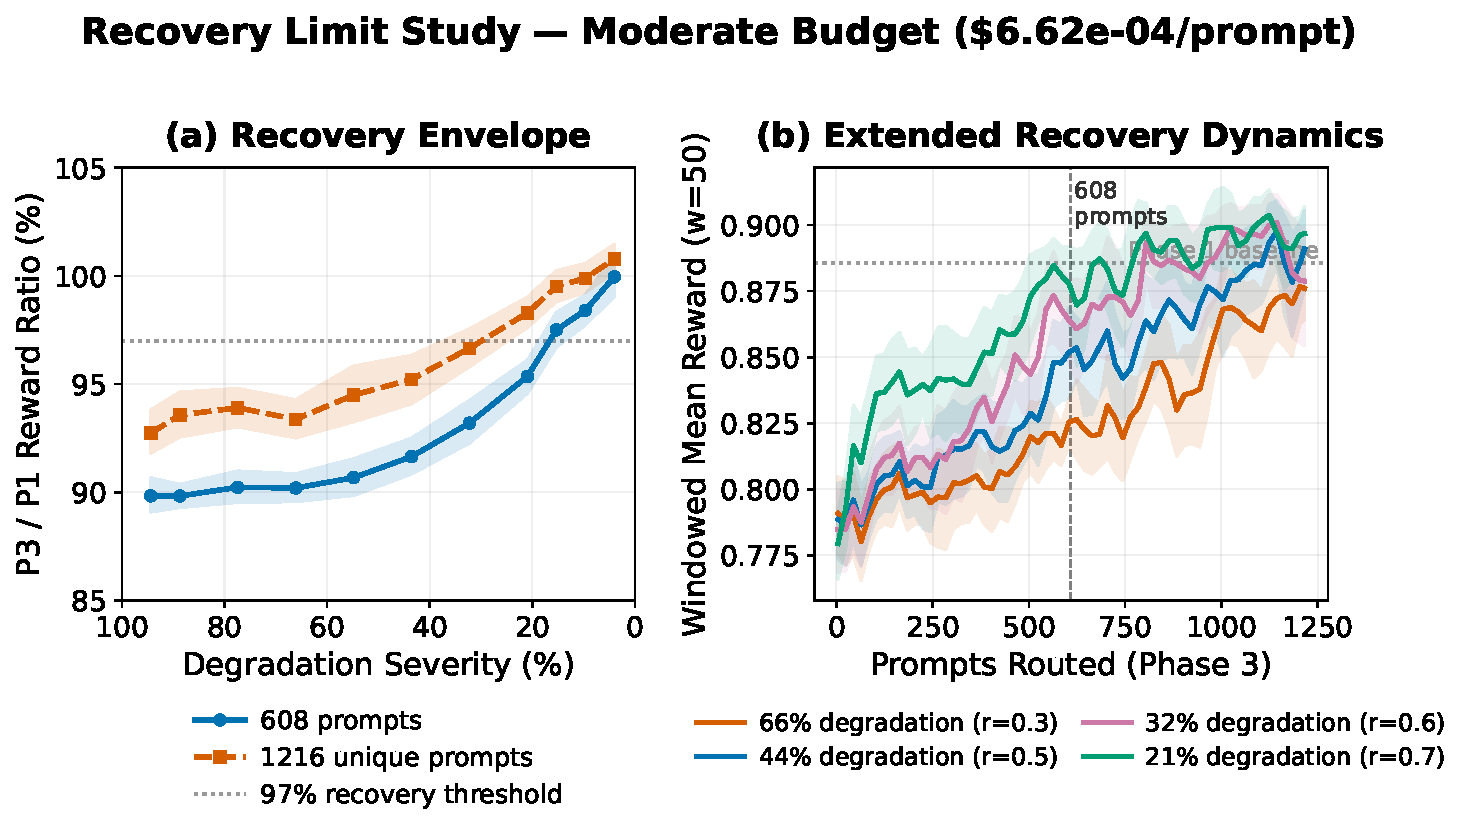
\includegraphics[width=\columnwidth]{../experiments/appendix/recovery_limit/results/recovery_limit.pdf}
\caption{Recovery limit under quality degradation (moderate budget, 20~seeds, 95\% bootstrap CI).
\textbf{(a)}~Recovery envelope: Phase~3/Phase~1 reward ratio vs.\ degradation severity for 608~prompts (blue, solid) and 1,800~prompts (orange, dashed).  The standard horizon achieves full recovery (${\geq}97$\%) up to ${\sim}18$\% degradation; the extended horizon shifts this boundary to ${\sim}44$\% and lifts even the most severe degradations from ${\sim}90$\% to ${\sim}95$\%.
\textbf{(b)}~Extended recovery dynamics for four representative degradation levels.  All trajectories converge toward the Phase~1 baseline (dotted), with milder degradations converging faster.}
\label{fig:recovery_limit}
\end{figure}
